\documentclass[dvisvgm,tikz]{standalone}
\usepackage{circuitikz}
\begin{document}
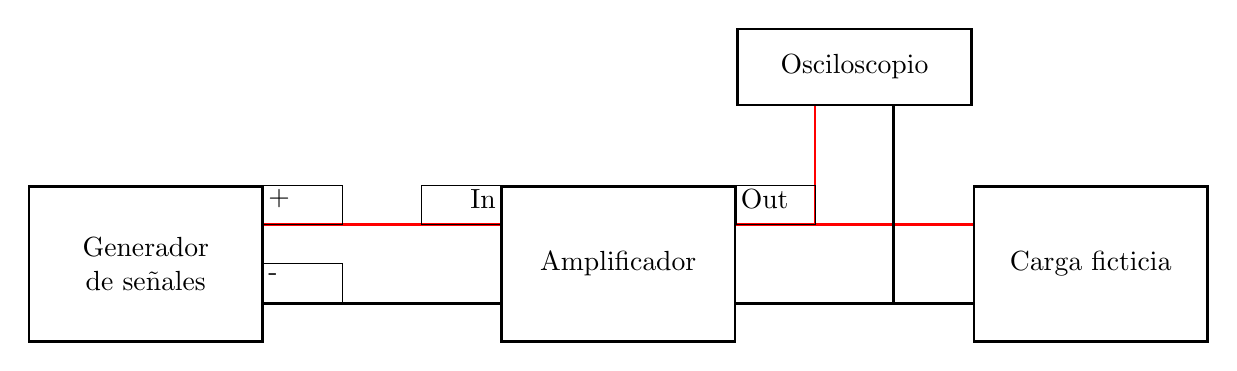
\begin{tikzpicture}
  \node[shape=rectangle, draw, line width=1pt, inner sep=0, minimum width=2.965cm, minimum height=1.965cm] at (1.5, 1){} node [anchor=center, align=center, text width=2.577cm, inner sep=5.5pt] at (1.5, 1){Generador de señales};
  \node[shape=rectangle, draw, line width=1pt, inner sep=0, minimum width=2.965cm, minimum height=1.965cm] at (7.5, 1){} node [anchor=center, align=center, text width=2.577cm, inner sep=5.5pt] at (7.5, 1){Amplificador};
  \node[shape=rectangle, draw, line width=1pt, inner sep=0, minimum width=2.965cm, minimum height=1.965cm] at (13.5, 1){} node [anchor=center, align=center, text width=2.577cm, inner sep=5.5pt] at (13.5, 1){Carga ficticia};
  \node[shape=rectangle, draw, line width=1pt, inner sep=0, minimum width=2.965cm, minimum height=0.965cm] at (10.5, 3.5){} node [anchor=center, align=center, text width=2.577cm, inner sep=5.5pt] at (10.5, 3.5){Osciloscopio};
  \draw[draw={rgb,255:red,255;green,0;blue,0}, line width=1pt] (3, 1.5) -- (6, 1.5);
  \draw[draw={rgb,255:red,0;green,0;blue,0}, line width=1pt] (3, 0.5) -- (6, 0.5);
  \draw[draw={rgb,255:red,255;green,0;blue,0}, line width=1pt] (9, 1.5) -- (12, 1.5);
  \draw[draw={rgb,255:red,0;green,0;blue,0}, line width=1pt] (9, 0.5) -- (12, 0.5);
  \draw[draw={rgb,255:red,255;green,0;blue,0}, line width=1pt] (10, 1.5) -| (10, 3);
  \draw[draw={rgb,255:red,0;green,0;blue,0}, line width=1pt] (11, 0.5) -| (11, 3);
  \node[shape=rectangle, draw, line width=0pt, inner sep=0, minimum width=1cm, minimum height=0.5cm] at (5.5, 1.75){} node [anchor=north east, align=right, text width=0.901cm, inner sep=1.4pt] at (6, 2){In};
  \node[shape=rectangle, draw, line width=0pt, inner sep=0, minimum width=1cm, minimum height=0.5cm] at (9.5, 1.75){} node [anchor=north west, align=left, text width=0.901cm, inner sep=1.4pt] at (9, 2){Out};
  \node[shape=rectangle, draw, line width=0pt, inner sep=0, minimum width=1cm, minimum height=0.5cm] at (3.5, 1.75){} node [anchor=north west, align=left, text width=0.901cm, inner sep=1.4pt] at (3, 2){+};
  \node[shape=rectangle, draw, line width=0pt, inner sep=0, minimum width=1cm, minimum height=0.5cm] at (3.5, 0.75){} node [anchor=north west, align=left, text width=0.901cm, inner sep=1.4pt] at (3, 1){-};
\end{tikzpicture}
\end{document}